\chapter{CUDAmino}
\label{sec:cudamino}

CUDAmino is a GPU accelerated \acf{MC} dMRI simulator based on the \ac{MC} simulator that is part of the Camino software package \cite{Cook2006,Hall2009}. 
The basic \acl{MC} \ac{dMRI} simulation algorithm outlined in \Cref{alg:MC_random_walk} does not change when adapting the simulations to run on the \ac{GPU}, however some changes are necessary to make the simulations efficient for the \ac{GPU}.

This section introduces CUDAmino, outlining the differences between CUDAmino and Camino as well as presenting some experiments assessing the performance of CUDAmino relative to Camino.

\section{CUDAmino design}
\label{sec:cudamino_design}
CUDAmino is, of course, designed to exploit the parallel nature of the \ac{GPU}.
Since each spin is simulated independently of all of the other spins, the problem is inherently parallel and we can use each execution thread to simulate a single spin.

The problem could also be parallelised along the time dimension, however that can lead to a problem known as a race condition.
A race condition occurs when the program tries to do two things at once, but one should rely on the other so they must be done in order.
In this instance, you could get one thread trying to take the $(t+1)^{\mathrm{th}}$ step before the $t^{\mathrm{th}}$ step is finished.
For this reason, CUDAmino is only parallelised along the number of spins.

Another potential pitfall of GPU simulations, mentioned in \Cref{sec:bg_gpu}, is thread divergence.
In particular, the while loop in \Cref{alg:MC_random_walk} could be a source of thread divergence.
Different threads will have spins in different locations, so may end up with different numbers of iterations of the loop to amend the step.
The impact of this will be accentuated by meshes with small structures where faces are close to each other, so there may be many multiple reflections.

In order to try and minimise thread divergence, CUDAmino follows the technique of Waudby and Christodoulou \cite{Waudby2011} who use rejection sampling.
The rejection sampling technique simply checks whether any given step has crossed a face and if it has, then the step is rejected and the spin does not move.
Provided the steps are small relative to the size of the structures in the substrate, the difference between rejection sampling and reflection is minimal\cite{Johannesson1996}.

Another consideration when designing CUDAmino, was to limit the number of unnecessary collision checks.
A complex mesh may have hundreds of thousands or millions of faces, if each step in the simulation has to check all faces, it will be unnecessarily slow.
The step should, ideally, only check for collisions with those faces which are nearby to it, in doing so it may be possible to reduce the number of collision checks from hundreds of thousand to a few tens of faces.

This problem of reducing the number of faces required for collision checks is a well studied problem in the field of ray-traced graphics rendering.
A number of spatial partitioning schemes have been developed to accelerate collision checks  such as the simple uniform grid \cite{Fujimoto1986,Amanatides1987}, octree \cite{Fujimoto1986} and \ac{BVH}\cite{Kay1986}. 

So far, aligning with the \ac{CPU} Camino implementation, CUDAmino uses a simple uniform grid acceleration scheme. In short, this uniformly subdivides the space in which the mesh sits, meaning that each step need only check collisions for the triangles within the subspace that the step goes through.

\begin{figure}[t]
  \centering
  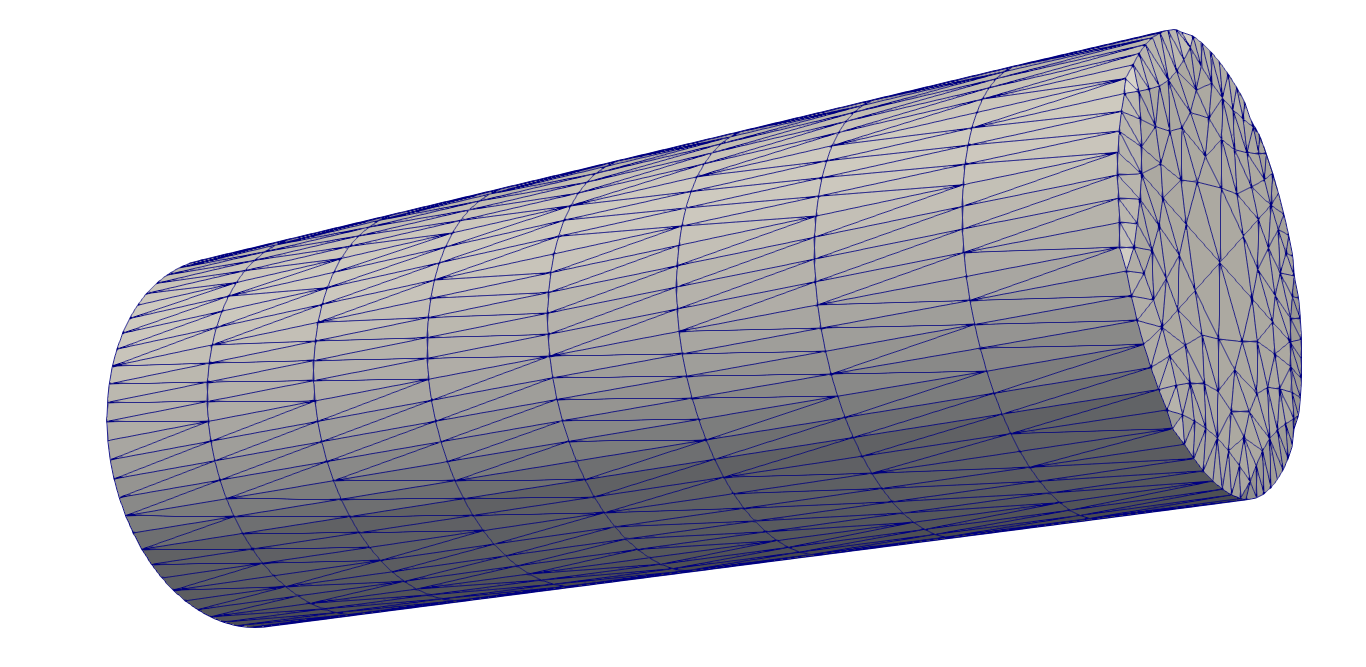
\includegraphics[width=0.7\textwidth]{figures/cudamino/cylinder.png}
  \caption{Cylinder mesh used for testing CUDAmino containing 1536 faces.}
  \label{fig:cudamino_cyl}
\end{figure}

\section{CUDAmino Experiments}
\todo[inline]{this section is work in progess, plan to complete this weekend}
In order to test CUDAmino's performance against Camino, two experiments were carried out.
Both experiments were carried out using a simple cylinder as shown in \Cref{fig:cudamino_cyl}, which has a radius of 0.9 $\mu$m and length of 5 $\mu$m and 1536 faces.

The first experiment investigated the effect of the number of timesteps on the resulting simulated signal.
As the number of timesteps increases, the step length decreases and the rejection sampling approach of CUDAmino should approach the reflection approach of Camino.

Simulations were run in both Camino and CUDAmino with $n = 10000$ spins and $t_{max} = 1000, 10000, 50000$.
Simulated \ac{dMRI} signals were generated using a standard \ac{PGSE} sequence with $\Delta = 12.5$ ms, $\delta = 1$ ms and $b$-value ranging from 0 to 19.5 mm$^2$/s.


\begin{figure}
  \centering
  \begin{subfigure}{0.49\textwidth}
    \centering
    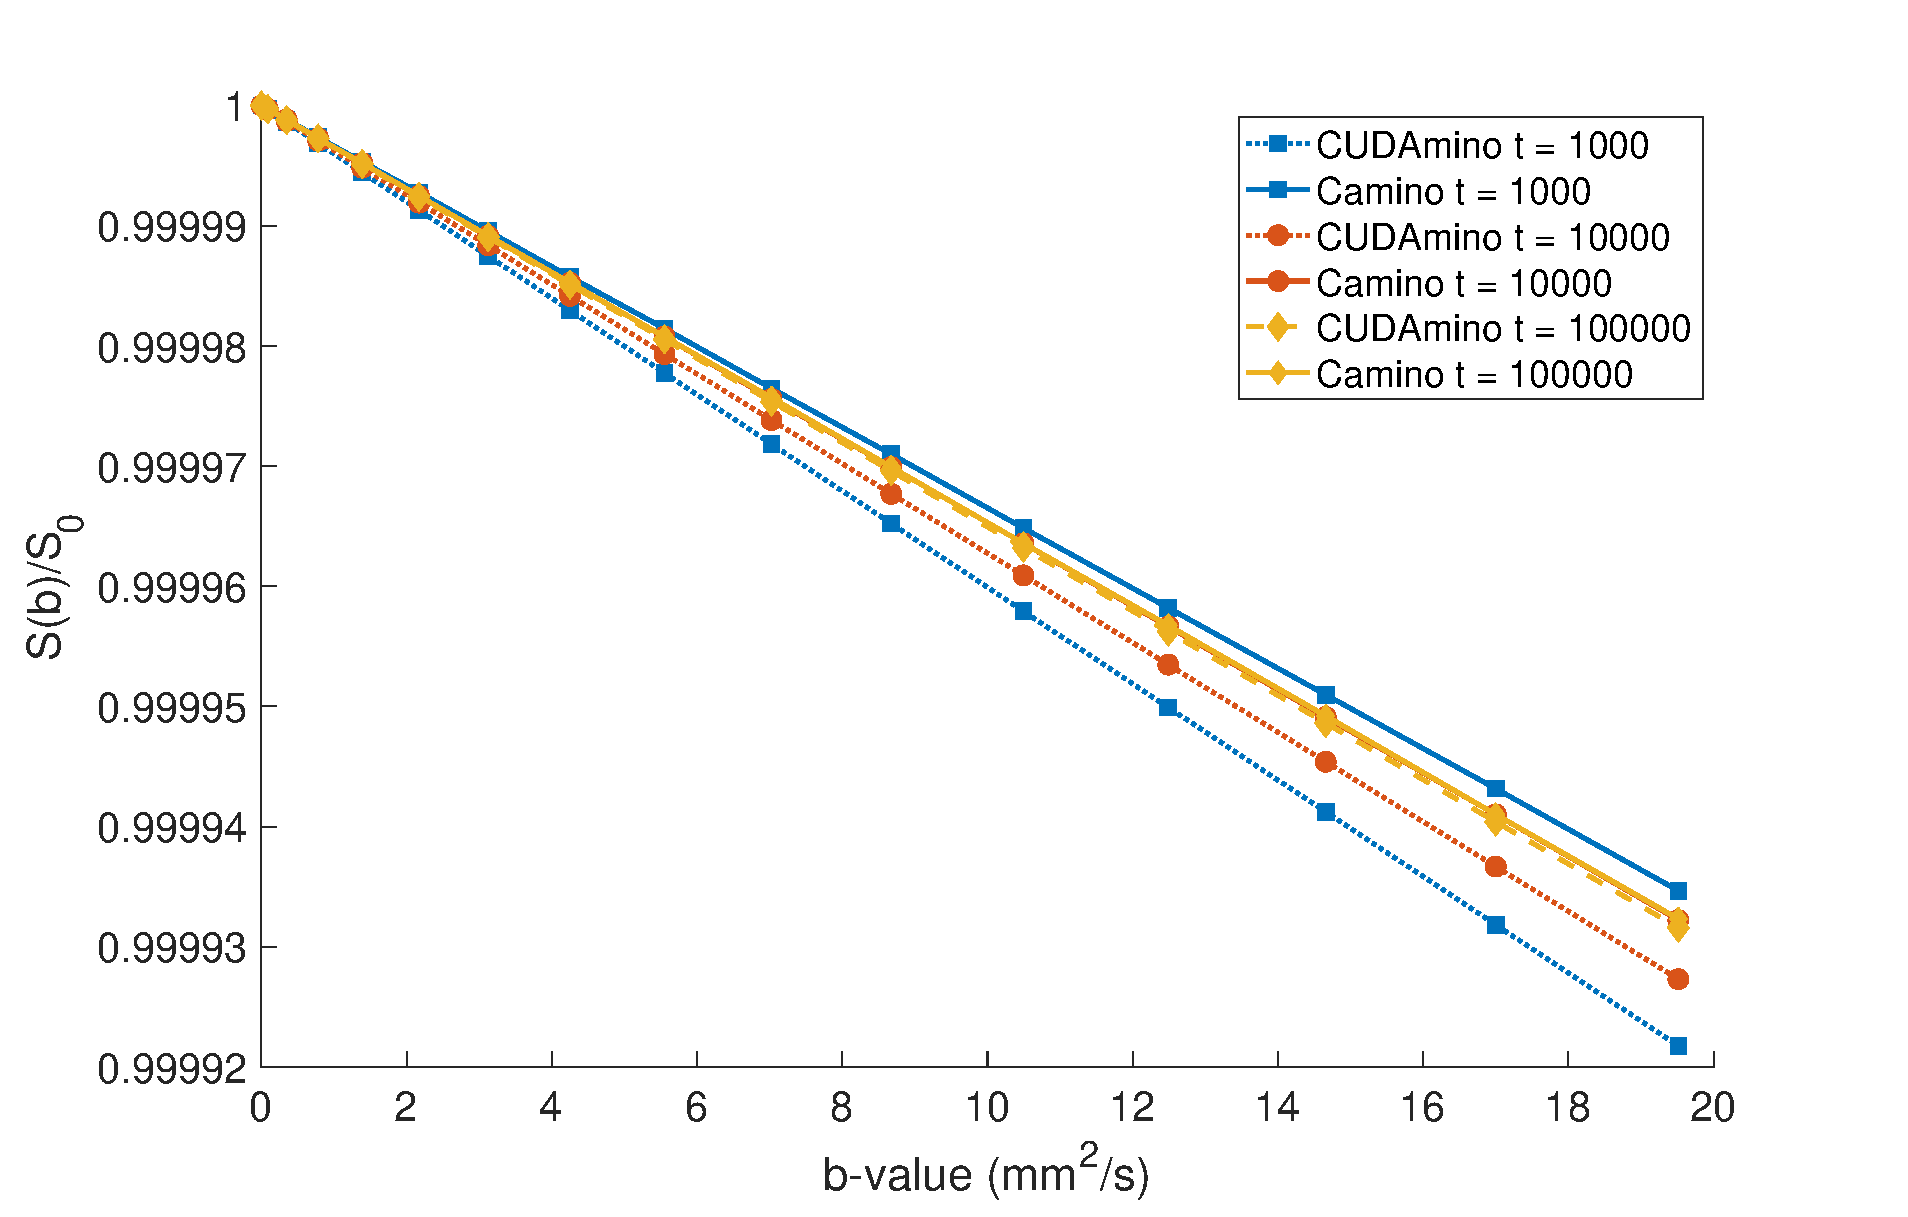
\includegraphics[width=\textwidth]{figures/cudamino/cyl_tmax.eps}
    \caption{}
    \label{fig:cyl_tmax_sig}
  \end{subfigure}
  ~
  \begin{subfigure}{0.49\textwidth}
    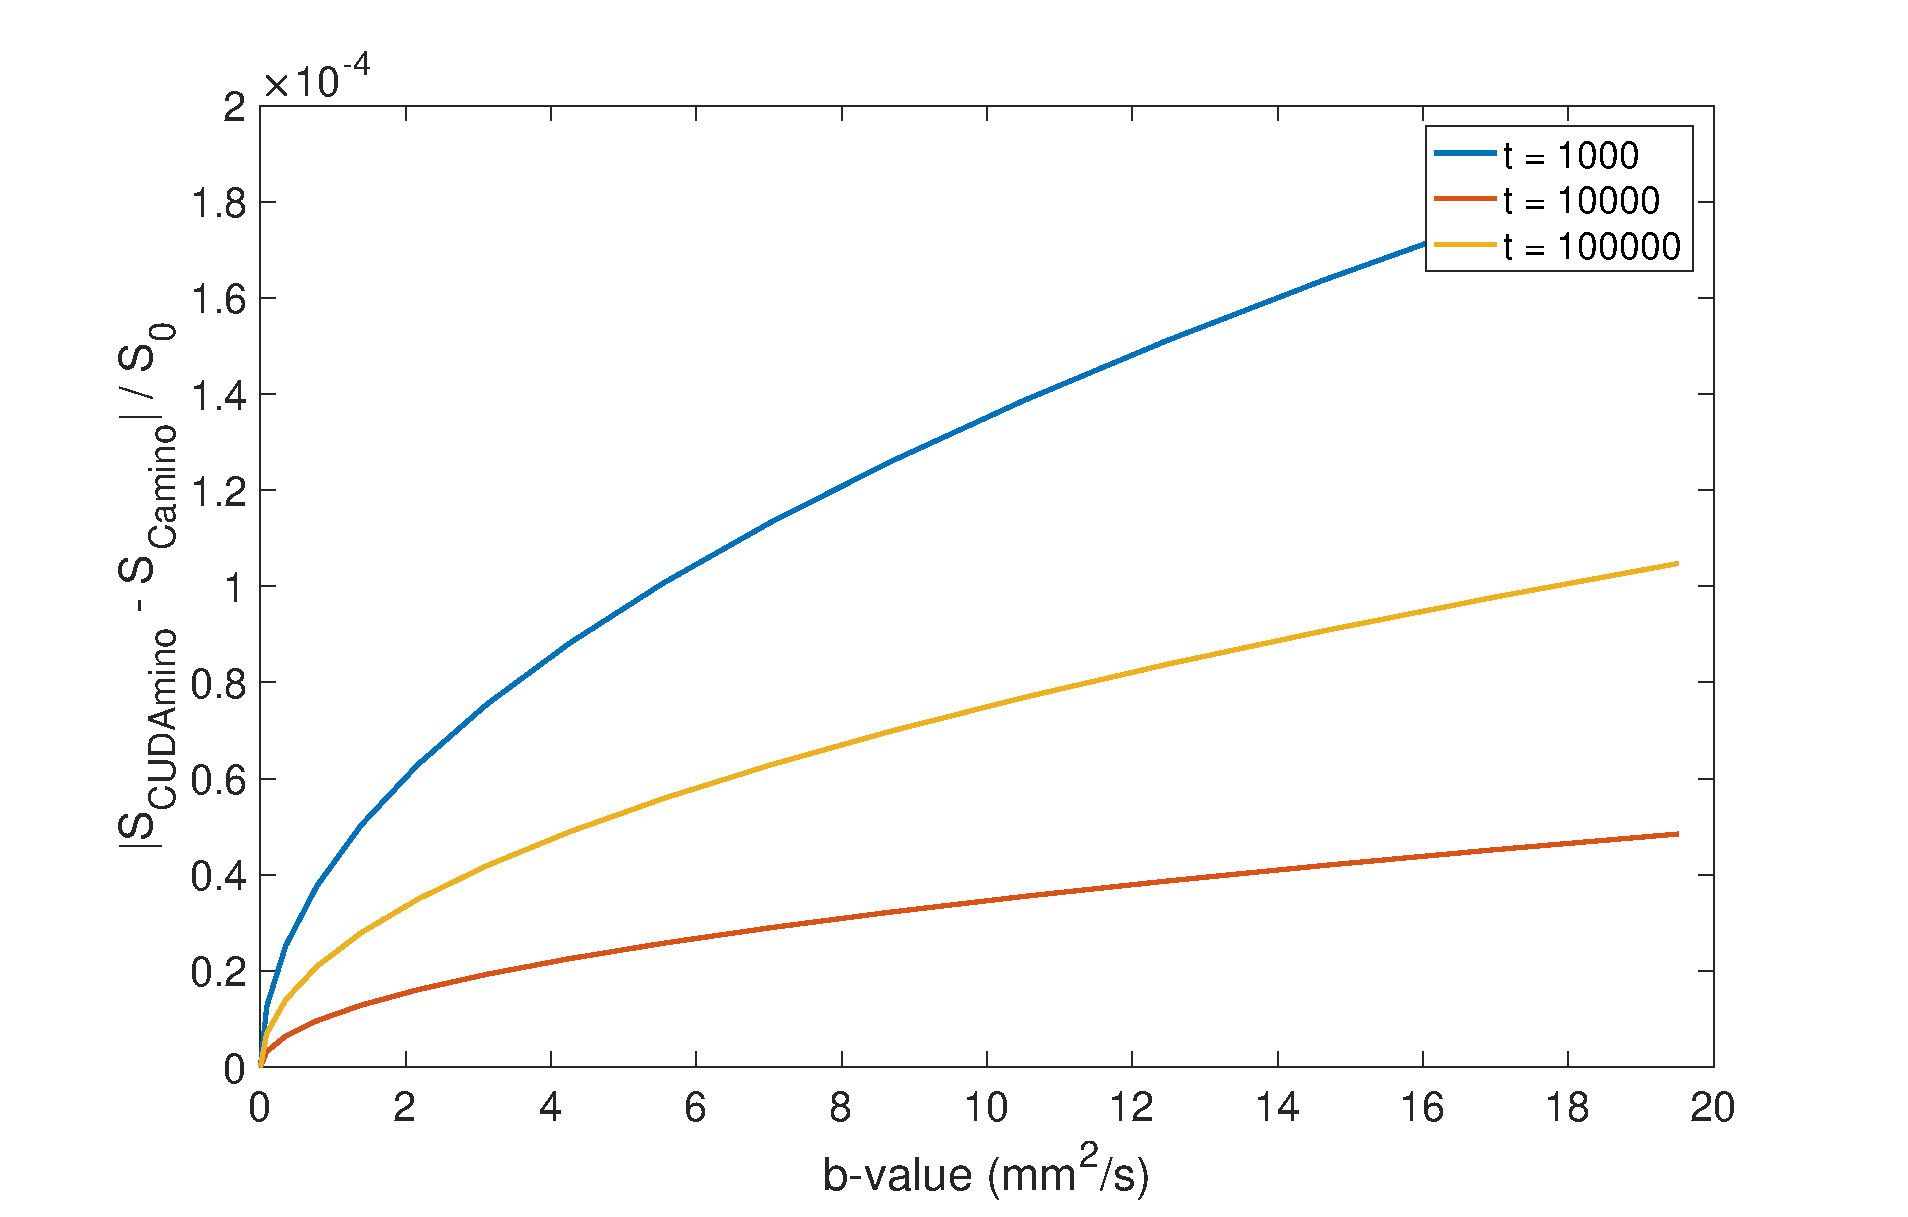
\includegraphics[width=\textwidth]{figures/cudamino/cyl_tmax_diff.eps}
    \caption{}
    \label{fig:cyl_tmax_diff}
  \end{subfigure}
  \caption{Cylinder tests varying $t_{max}$. a) The simulated \ac{dMRI} signals and b) The difference between CUDAmino and Camino signals.Cylinder tmax tests}
  \label{fig:cyl_tmax}
\end{figure}

\Cref{fig:cyl_tmax} shows the results of the tests varying the number of timesteps. \Cref{fig:cyl_tmax_sig} shows the simulated \ac{dMRI} signal for both CUDAmino and Camino, while \Cref{fig:cyl_tmax_diff} shows the relative difference between the CUDAmino and Camino signals.
The difference between the simulated signals is smallest with the highest number of timesteps, though the difference between the CUDAmino and Camino is small relative to the $S_0$ signal for all timesteps. 

A similar experiment was carried out, varying the number of spins rather than the number of timesteps.
In this case, $t_{max}$ was fixed to 5000 and $n = 1000, 10000, 100000$.
The same \ac{PGSE} sequence parameters were used.

\Cref{fig:cyl_nspin} shows the results of the simulations with different numbers of spins. \Cref{fig:cyl_nspin_sig} shows the simulated signal for both CUDAmino and Camino.
\Cref{fig:cyl_nspin_diff} shows the difference between CUDAmino and Camino. In this case, an increased number of spins increases the difference between the simulated signals.
This suggest some systematic difference between CUDAmino and Camino which is greater with larger numbers of spins.
This could be due to the differences between rejection sampling and reflection building up more and more with increased numbers of spins, however this requires further investigation. 

\Cref{tab:cyl_tmax_time,tab:cyl_nspin_time} show the differences in running time between Camino and CUDAmino for both experiments.
In both cases, CUDAmino executes significantly faster, with 60-100$\times$ speedup in the $t_{max}$ case and a best case improvement of 15$\times$ for the $n$ test. 


\begin{figure}
  \centering
  \begin{subfigure}{0.49\textwidth}
    \centering
    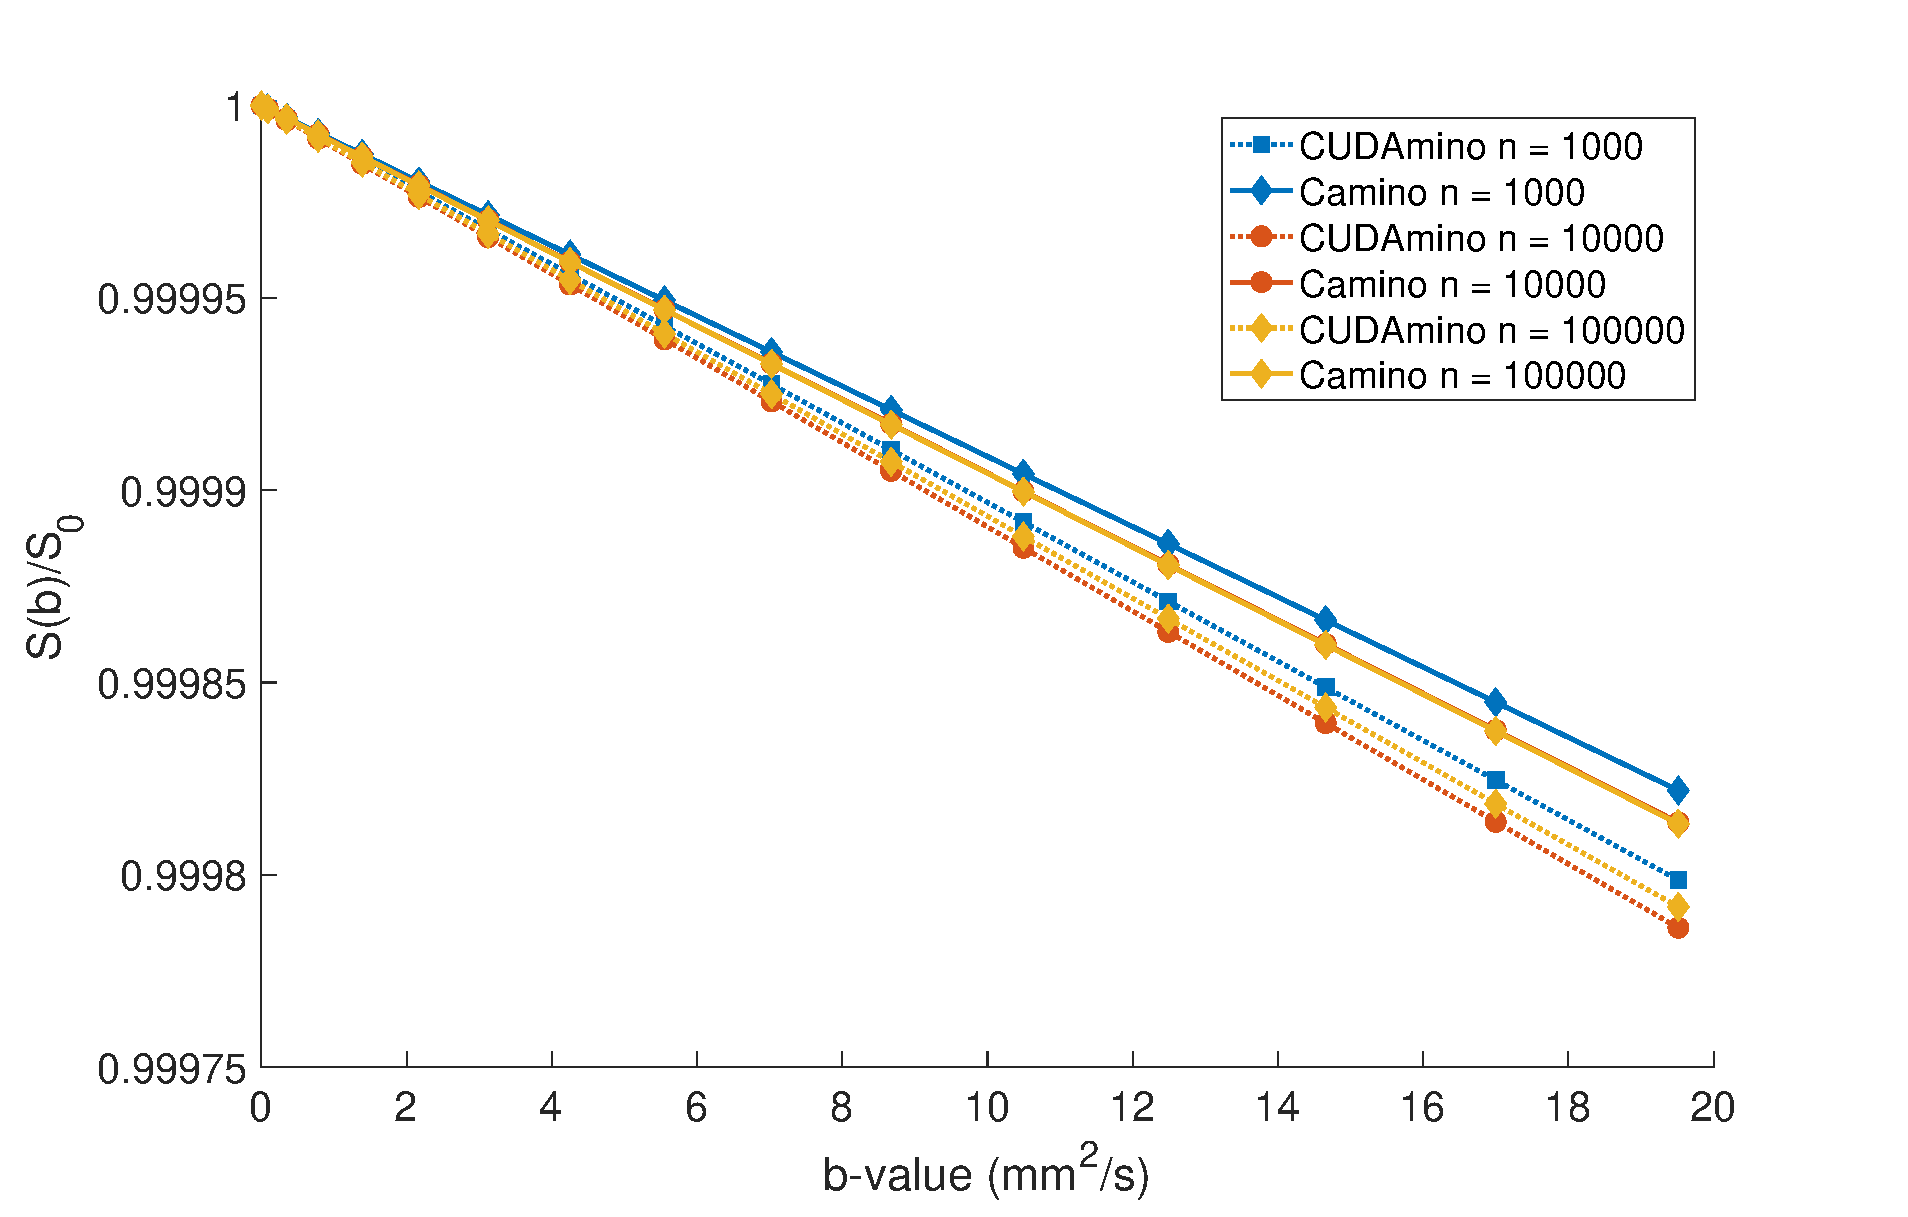
\includegraphics[width=\textwidth]{figures/cudamino/cyl_nspin.eps}
    \caption{}
    \label{fig:cyl_nspin_sig}
  \end{subfigure}
  ~
  \begin{subfigure}{0.49\textwidth}
    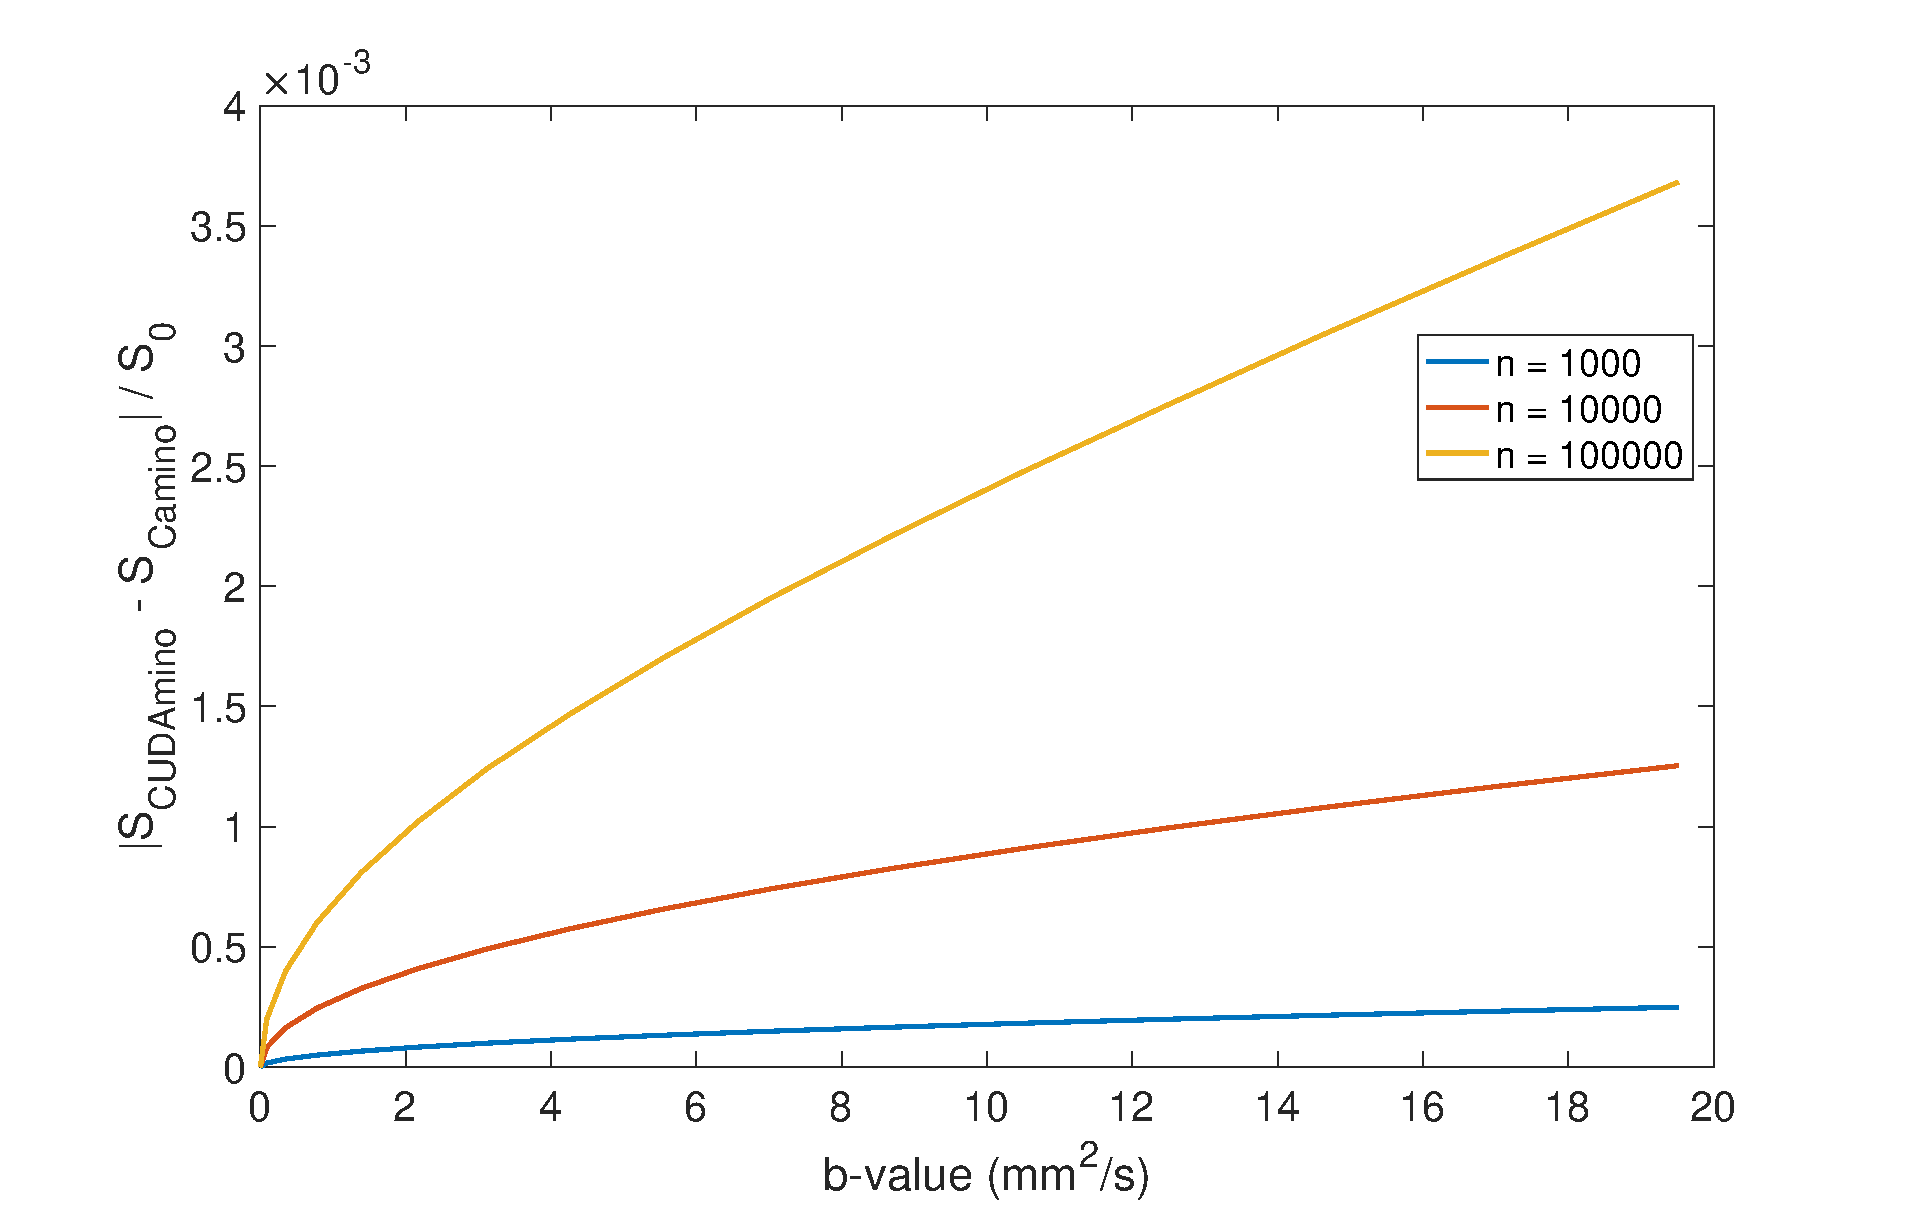
\includegraphics[width=\textwidth]{figures/cudamino/cyl_nspin_diff.eps}
    \caption{}
    \label{fig:cyl_nspin_diff}
  \end{subfigure}
  \caption{Cylinder tests varying $n$. a) The simulated \ac{dMRI} signals and b) The difference between CUDAmino and Camino signals.}
  \label{fig:cyl_nspin}
\end{figure}


\begin{table}
  \centering
  \begin{tabular}{|c|c|c|}
    \hline
    $t_{max}$ & Camino Time (s) & CUDAmino Time (s)\\\hline
    1000 & 317.33& 3.0951\\
    10000 & 1744.4& 24.547\\
    50000 & 7333.4& 112.03\\\hline
  \end{tabular}
  \caption{Running time comparison of Camino and CUDAmino for experiments with variable $t_{max}$}
  \label{tab:cyl_tmax_time}
\end{table}


\begin{table}
  \centering
  \begin{tabular}{|c|c|c|}
    \hline
    $n$ & Camino Time (s) & CUDAmino Time (s)\\\hline
    1000 & 9.0979 &7.0987 \\
    10000 & 94.402 &7.2175\\
    100000 & 1124.5 &80.821\\\hline
  \end{tabular}
  \caption{Running time comparison of Camino and CUDAmino for experiments with variable $n$}
  \label{tab:cyl_nspin_time}
\end{table}




\section{Discussion and Conclusion}
\label{sec:cudamino_discussion}
\todo[inline]{again, this section is WIP}

CUDAmino, as presented here, still has some way to go to fully replicate Camino's diffusion simulations.
There are a number of features lacking, such as permeability and full reflections, however this represents a good first step towards a fully-featured GPU \ac{dMRI} simulator.

As shown in \Cref{fig:cyl_tmax,fig:cyl_nspin}, the difference between the simulated signals in CUDAmino and Camino is small in the simple scenario presented.
The is a promising result as it shows that CUDAmino is able to match the results of Camino well. There should be further investigation into the exact differences between the two, however, since the increasing error as $n$ increases (\Cref{fig:cyl_nspin_diff}) is troubling, as large, complex substrates will require a large number of spins.  

The performance boost that CUDAmino has over Camino, running simulations 15-100$\times$ faster shows the promise that CUDAmino has in making \ac{dMRI} simulations much more efficient. 

%%% Local Variables:
%%% mode: latex
%%% TeX-master: "../main"
%%% End:
